\section{Trasowanie Cebulowe}\paragraph{}
Trasowanie Cebulowe jest techniką pozwalającą na anonimową komunikację w~Internecie. Do jej działania wykorzystystywana jest grupa węzłów przez które przekierowywana jest wiadomość, zanim trafi do docelowego odbiorcy. Zasada działania polega na tym, że nadawca wiadomości pobiera listę węzłów pośredniczących, a~następnie wybiera kilka spośród nich (węzły te będą tworzyć obwód przez który będzie pośredniczona przesyłana wiadomość). Następnie szyfruje on wielokrotnie dane, które mają trafić do odbiorcy. Szyfrowanie odbywa się za pomocą kluczy kolejnych węzłów tworzących obwód w~odwrotnej kolejności niż się w~nim znajdują (najpierw do szyfrowania zostaje użyty klucz pierwszego węzła, a~na końcu klucz węzła znajdującego się na końcu obwodu). Zaszyfrowana wiadomość zostaje wysłana do pierwszego węzła, który odszyfrowuje ją, co powoduje odkrycie następnego węzła do którego ma trafić wiadomość. Wiadomość zostaje przekazywana do kolejnych węzłów, które zdejmują kolejne warstwy szyfru, do momentu aż trafi do ostatniego węzła, który zdejmuje najgłębszą warstwę szyfru i~przekazuje wiadomość w~oryginalnej postaci do docelowego odbiorcy. Dzięki takiemu systemowi przesyłania pakietów niemożliwe jest ustalenie całej trasy przesyłanego pakietu. Każdy z~węzłów zna tylko dwóch swoich sąsiadów, pierszy węzeł zna nadawcę, lecz nie wie jaka jest treść przesyłanej wiadomośći, a~ostatni zna odbiorcę, ale nie zna nadawcy wiadomości.

Rysunek \ref{rys:onion_diagram} przedstawia wygląd wiadomości, która zostaje przesłana przez obwód składający się z~trzech węzłów. Kolor niebieski oznacza warstwę szyfru utworzoną za pomocą klucza węzła, znajdującego się na początku obwodu, a~czerwony warstwę szyfru utworzoną za pomocą klucza ostatniego węzła. Najgłębsza (szara) warstwa wiadomości oznacza niezaszyfrowane dane, które mają trafić do docelowego hosta.
\begin{figure}
 \centering
 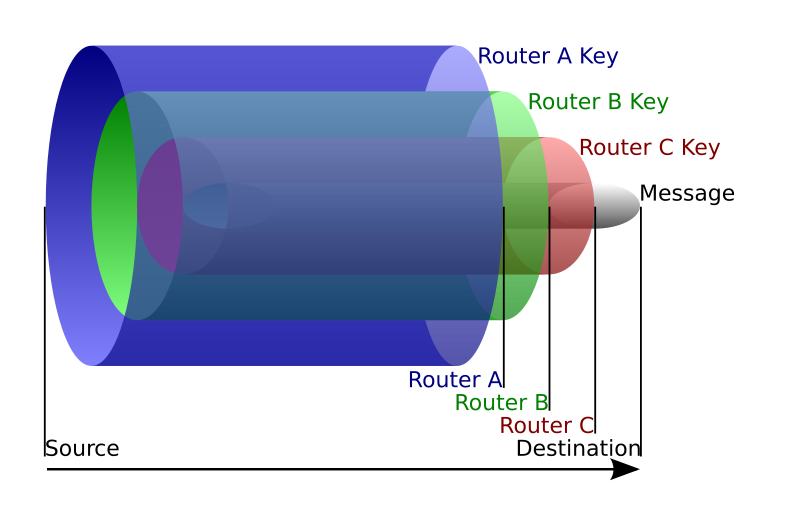
\includegraphics[width=\textwidth]{onion_diagram}
 \caption[Caption for LOR]{Diagram przedstawiający przykładową wiadomość przesyłaną przez obwód.\footnotemark}
 \label{rys:onion_diagram}
\end{figure}
\footnotetext{\url{https://upload.wikimedia.org/wikipedia/commons/e/e1/Onion_diagram.svg}}

\subsection{Komórki}\paragraph{}
Przesyłaną jednostką danych w~Trasowaniu Cebulowym jest tzw. komórka. Ma ona stałą długość 512 bajtów i~składa się z~nagłówka oraz przesyłanej treści. Długość nagłówka jest uzależniona od typu komórki. Może mieć on 3 lub 14 bajtów. Najważniejszymi składowymi nagłówka jest identyfikator obwodu oraz polecenie. Rysunek \ref{rys:cell} przedstawia wygląd komórki.

Pierwsze 2 bajty są zajmowane przez wcześniej wspomniany identyfikator obwodu. Jest on wymagany, gdyż w~pojedyńczym połączeniu pomiędzy poszczególnymi węzłami może zostać ustanowionych wiele obwodów\footnote{czym jest obwód} i~każdy węzeł\footnote{czym jest węzeł} musi wiedzieć do którego z~nich należy komórka.

Kolejny zajmowany bajt przeznaczony jest na polecenie, dzięki któremu węzeł, który otrzyma komórkę, będzie w~stanie zinterpretować ją w~odpowiedni sposób. Wszystkie polecenia można podzielić na dwa typy, kontrolne oraz przekazujące. Do tych pierwszych należą \textit{padding}, \textit{create} oraz \textit{destroy}. Służą one kolejno do utrzymywania połączeń, ustanawiania nowych obwodów oraz niszczenia ich, z~koleji poleceniem mówiącym nam o~tym, że mamy do czynienia z~komórką przekazującą jest \textit{relay}.

Struktura komórki posiadającej polecenie przekazujące różni się od komórek z~poleceniem kontrolnym tym, że pierwsze 11 bajtów treści komórki traktowane jest jako rozszerzenie jej nagłówka. Pierwsze 2 bajty tego rozszerzenia przeznaczone są na identyfikator strumienia, który jest wymagany ze względu na to, że pojedyńczy strumień może zostać zmultipleksowany na wiele obwodów i~potrzebny jest mechanizm pozwalający odróżnić do jakiego strumienia w~obwodzie należy komórka. Kolejne 6 bajtów zajmuje suma kontrolna, stworzona za pomocą funkcji skrótu SHA-1, pozwalająca na sprawdzenie integralności przesyłanych danych. Kolejne pole nagłówka określa długość przesyłanej treści, a~ostatni bajt określa odpowiednie polecenie komórki przekazującej. Do wykorzystywanych poleceń należą:

\begin{itemize}
\setlength\itemsep{0mm}
 \item \textit{relay data} - przesyłanie danych w~strumieniu
 \item \textit{relay begin} - otwarcie strumienia
 \item \textit{relay end} - bezpieczne zamknięcie strumienia
 \item \textit{relay teardown} - zamknięcie uszkodzonego strumienia
 \item \textit{relay connected} - powiadomienie proxy nadawcy o~rozpoczęciu przekazywania
 \item \textit{relay extend} - rozszerzenie obwodu o~nowy węzeł
 \item \textit{relay extended} - potwierdzenie rozszerzenia obwodu
 \item \textit{relay truncate} - zamknięcie części obwodu
 \item \textit{relay truncated} - potwierdzenie zamknięcia części obwodu
 \item \textit{relay sendme} - kontrola przeciążenia
 \item \textit{relay drop} - implementacja atrap dalekiego zasięgu
\end{itemize}

\begin{figure}
 \centering
 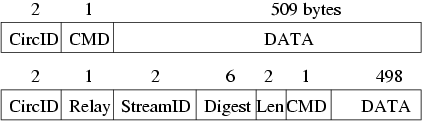
\includegraphics[width=\textwidth]{cell}
 \caption[Caption for LOR]{Struktura komórki Trasowania Cebulowego typu kontrolnego (u góry) oraz przekazującego.\footnotemark}
 \label{rys:cell}
\end{figure}
\footnotetext{https://svn.torproject.org/svn/projects/design-paper/tor-design.html}

\subsection{Proces tworzenia obwodu}\paragraph{}
Każde dwa węzły w~obwodzie są ze sobą połączone przy użyciu protokołu TLS. Proces tworzenia obwodu przebiega w~sposób iteracyjny. Załóżmy, że Alice jest nadawcą znajdującym się na początku obwodu, pierwszym węzłem jest Bob, a~drugim w~kolejności Carol:
\begin{enumerate}
 \item Alice w~celu utworzenia obwodu wysyła 
\end{enumerate}


\subsection{}